%!TEX root = ../../perdespassup.tex

\chapter[Persuasive Design for Password Support (P4P)]{Persuasive Design for \\ Password Support}\label{chap:perdespassup}
Having reviewed the literature (Part \ref{part:related_work}), and explored both the problem space (Part \ref{part:problem_space}) and design space (Part \ref{part:design_space}), we can now take a step back and synthesize common streams, results, and lessons learned. 
% GOAL: Support users in any kind of task that involves passwords. 
As a result, this chapter presents a new framework for researchers and designers to find and evaluate persuasive strategies that support users in any task that involves passwords. 
% Why is this necessary? / Motivation: covariates disregarded
We can find numerous research papers that evaluate a specific aspect without much context information or covariates. For instance, many types of password meters have been designed and evaluated, but most focused on measuring impact in the form of resulting password strength and usability metrics alone. However, aspects like user's preexisting mental models of password strength or the deployment environment were often untouched. At the same time, it is important to focus on the users and choose the support strategy that works best for them under a given configuration of environmental variables. 
% motivation: previous approaches might have lacked structure leading to lower efficacy 
Moreover, we find that many persuasive strategies stay below their potentials \cite{Renaud2017LessonsLearnedNudges}, or show unexpected effects (see Chapter \ref{chap:decoy}). Therefore, I establish a design process to avoid past shortcomings in nudging effects and to aid strategic decision-making for persuasive design. 


The \textbf{Persuasive Design for Password Support} (\textbf{P4P}) framework broadens the view on exploring and designing support systems (see Figure \ref{fig:p4p:passup}). It is divided into two ``lenses'' for the task. The ``research lens'' covers the ever-changing, heterogeneous environmental factors in usable password authentication and how to elicit them. It helps explain \textit{why} users act in certain ways and can provide pointers as to \textit{why} we should try to change the current state. The ``design lens'' assesses the status quo of password authentication and helps find solutions of different obtrusiveness levels (first stage), i.e. \textit{what} should be the focus of a new persuasive strategy. The second stage defines a user-centered process to implement when the required level of support has been decided. It aids in finding out \textit{how} the persuasive strategy should look. In the following, I explain these elements and show a design exercise where I apply the framework to create a novel approach for a password manager. 

%there won't be a formula like ``if X then use strategy Y'' (magic wand strategy). Rather, one needs to give different aspects some thought. 

%%%%%%%%%%%%%%%%%%%%%%%%%%%%%%%%%%%%%%%%
%
% FRAMEWORK FIGURE
%
%%%%%%%%%%%%%%%%%%%%%%%%%%%%%%%%%%%%%%%%
\begin{figure}[!htbp]
	\centering
	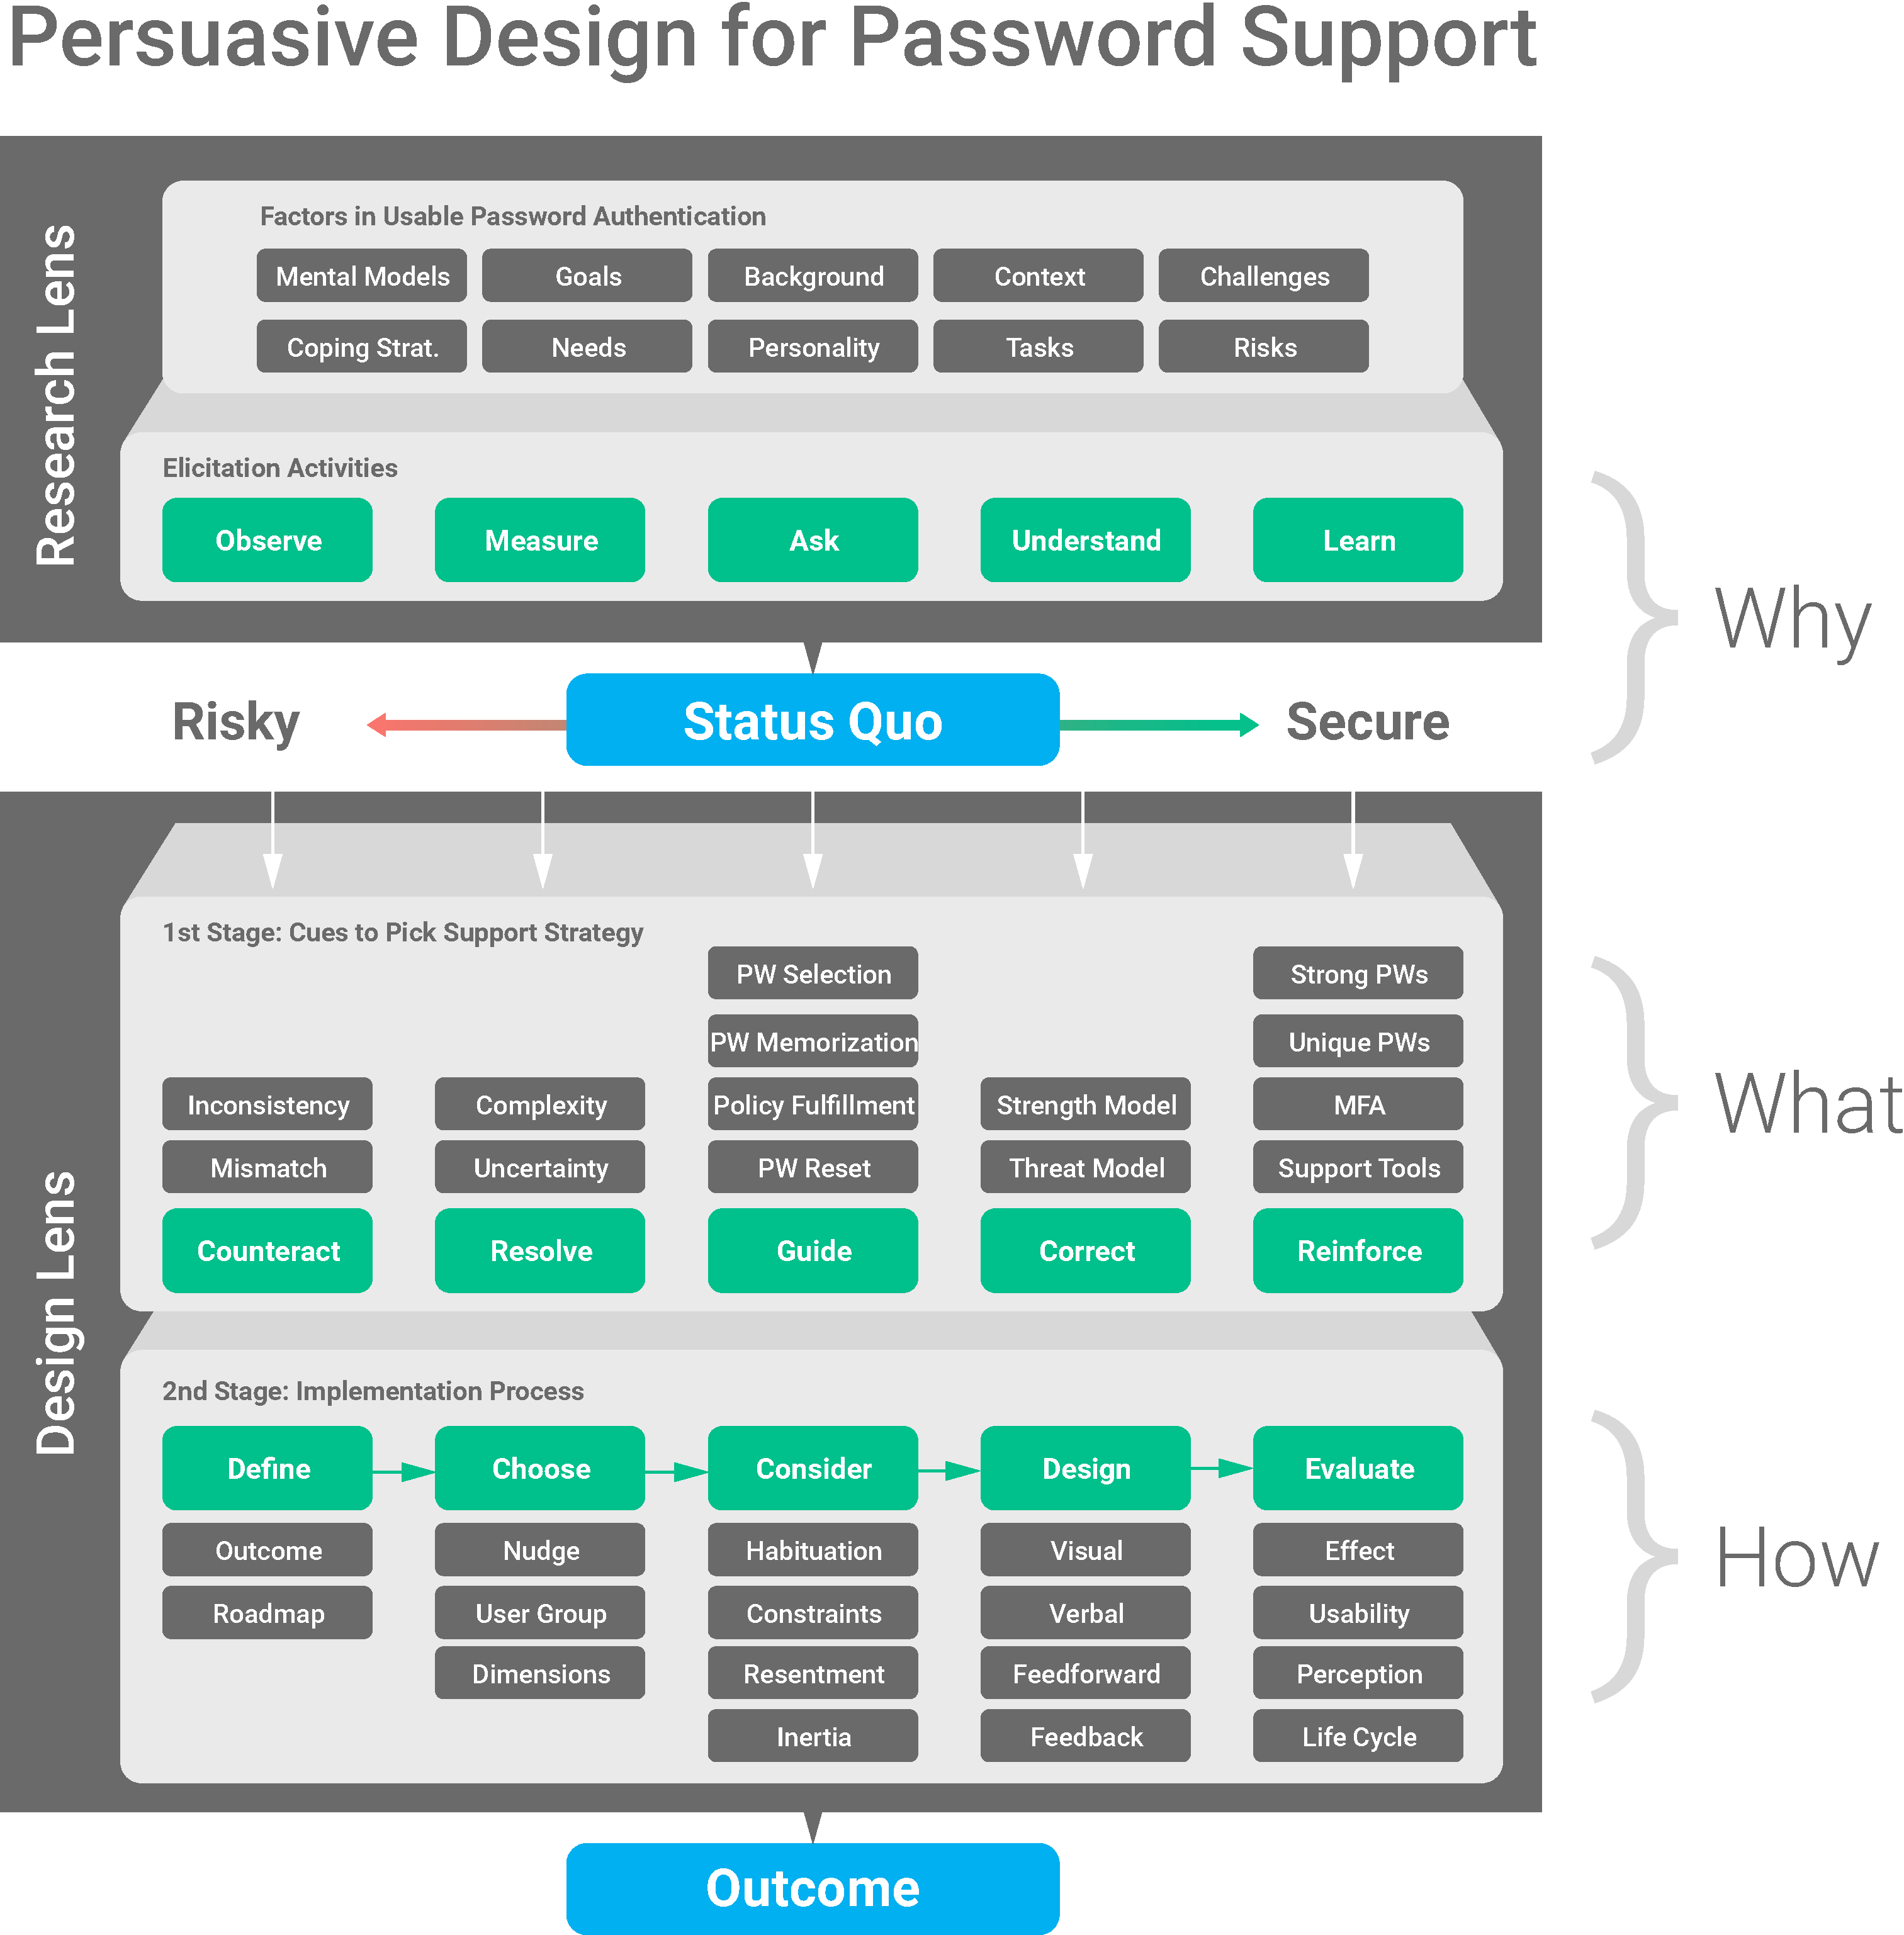
\includegraphics[width=\linewidth]{figures/pst/PerdesPassup}
	\caption{\label{fig:p4p:passup} Persuasive Design for Password Support (P4P) is a specialized design framework for strategic intervention development.}
\end{figure}

%%%%%%%%%%%%%%%%%%%%%%%%%%%%%%%%%%%%%%%%
%
% RESEARCH LENS
%
%%%%%%%%%%%%%%%%%%%%%%%%%%%%%%%%%%%%%%%%
\section{Research Lens}
% Assumptions -- reduce assumptions. 
The first step to create a novel persuasive support strategy is to elicit a number of factors that are involved in usable password authentication. Some of them have been addressed in previous research, e.g. coping strategies, while others are a direct consequence of the findings presented in this thesis (e.g. mental models or personality). 
% table
Researchers can try to answer the following questions to obtain an overview of the status quo of risky and secure factors:
%\begin{tabular}{p{14cm}l}

\vspace*{0.5cm}
\noindent
\resizebox{\linewidth}{!}{
\begin{tabular}{|p{14cm}l|}
	\hline
	\textbf{Question} & \textbf{P4P Element} \\
	What are current mental models, e.g. of password strength or support tools? & Mental Models\\
	How do different user groups cope with passwords? & Coping Strategies \\
	What are users trying to achieve they authenticate? & Goals \\
	What are the dimensions of user needs in this context, also in regard to support? & Needs \\
	How does demographic background impact password attitudes and behavior? & Background\\
	How much is personality visible in attitudes and behavior regarding authentication? & Personality \\
	What is the broader context of the task, e.g. personal vs. work environment? & Context \\
	What tasks does the user need to perform to reach their goals? & Tasks \\
	What are the challenges that different users face in the task? & Challenges \\
	What risks are there if the user acts insufficiently secure? & Risks\\\hline
\end{tabular}
}
\vspace*{0.5cm}

Some of these questions already hint at the dynamics of certain factors. For instance, users' mental models about threats might adapt over time, e.g. after falling prey to a phishing scam. Adoption rates of password managers are also volatile and the percentage of people relying on them certainly affects the type of novel support strategies one can implement. Although many questions and aspects can be answered by desk research methods, the dynamic evolution of the factors requires ongoing elicitation. Thus, traditional empirical research methods can be used to \textbf{observe} behavior and problems, \textbf{measure} interactions, explicitly \textbf{ask} users about certain aspects, \textbf{immerse} in the context of different user groups, and \textbf{learn} from all these activities. The result of this exploration is a detailed picture of the status quo. 

%%%%%%%%
% Questions
%%%%%%%
%\section{Guiding Support Strategies}

\subsubsection{Roadmap}
\begin{tabular}{p{14cm}l}
	What is the desired outcome? & Outcome \\
	How difficult is it to achieve and why? & Difficulty \\
	How big would the impact be? & Impact \\
	How important is it to achieve this outcome? & Importance
\end{tabular}

\subsubsection{Strategy}
\begin{tabular}{p{14cm}l}
	What exactly is the strategy based on? & Foundation\\
	Why is it expected to work? & Support\\
	What stage(s) in the password life cycle does it target? & Stage \\
	What is the specific context? & Context \\
	Are there other ways to achieve the same effect? & Alternatives \\
	Who is the target user group? & User Group\\
	How does the strategy relate to other frameworks? & Relationships\\
	Is it a one-off effort or continuous support? & Time-Scale \\
\end{tabular}

\subsubsection{Prerequisites}
\begin{tabular}{p{14cm}l}
	What are the dimensions of user needs in this context? & Needs \\
	How can the needs be met by the strategy? & Match \\
	What are the characteristics of the strategy? & Characteristics\\
	What are the minimum abilities that the user needs to have? & Abilities\\
\end{tabular}

\subsubsection{Risks}
\begin{tabular}{p{14cm}l}
	Will users get habituated to the strategy and is this good or bad? & Habituation\\
	How would the strategy interfere with other solutions? & Interference\\
	Does the strategy require too much effort from the users? & Effort\\
\end{tabular}

\subsubsection{Evaluation}
\begin{tabular}{p{14cm}l}
	How is the strategy going to be evaluated? & Method\\
	Is it possible to triangulate methods? & Triangulation\\
	What are the metrics to track impact? & Metrics	
\end{tabular}



\subsubsection{Status Quo}
% subjective assessment, but there are certain cues that
The status quo is a snapshot of the levels and relative importance of the factors that contribute to usable password authentication. Although the data elicitation should be generalizable and objective, the judgment of the result is not. It is up to researchers to collaboratively assess how risky a certain user group behaves in various contexts. Here, the framework posits that some aspects that have traditionally been considered ``risky'' behavior need to be seen in a different light as attacks and countermeasures evolve. This follows the argumentation of Florêncio, Herley, Bonneau, and Van Oorshot among others \cite{Florencio2016CommACM, Herley2012PersistenceOfPasswords, Bonneau2012ReplacePasswords}. For instance, not all passwords need to withstand offline attacks. Therefore, it is unnecessary to nudge users to create passwords that would withstand them, because the usability drawbacks are unbearable for many users in most situations. The status quo thus informs the level of intervention in the subsequent design phase.

\section{Design Lens}
% pattern: If <user group> who <other factors | specific needs> do <cue>, then this can be seen as <risky|secure> and justifies <intervention>. 
The second half of the framework consist of two distinct phases: 1) Identifying the right level of support and 2) creating novel persuasive solutions. The first stage is strongly influenced by the results of the status-quo analysis. 

\subsubsection{Cues to Pick the Right Support Strategy} The interventions are ordered by their level of justifiable obtrusiveness. On the left, very risky behavior should be tried to \textbf{counteract}. The risk-level assessment is context dependent and can be read from the status quo analysis, where context is one dimension. We can read the elements like ``if X then Y'' in vertical direction. In particular, the framework follows this pattern:

\vspace*{1em}
\noindent
\fbox{
	\hspace{0.03\linewidth}
	\centering
	\parbox[c][2cm]{0.9\linewidth}{
		If \textit{<user group>}, who are \textit{<list of factors>}, do \textit{<specific action>}, then this can be seen as \textit{<risky or secure>} and justifies \textit{<intervention level>}.
	}
	\hspace{0.03\linewidth}
}
\vspace*{1em}

\noindent For example, the framework suggests that if \textit{users of online web-services} show \textit{clear patterns of inconsistent reuse}, i.e. reusing a password from a high-value account on a low-value website, then this is \textit{risky }behavior and should be \textbf{counteracted} with obtrusive strategies. The same goes for mismatches of account value and password strength. Other aspects can be \textbf{resolved} with less user-involvement and obtrusion. For instance, if status quo analysis shows that current password policies in companies are too complex, they should thus be replaced by simpler versions. Decisions under uncertainty, e.g. when a user needs to assess how valuable an account is, can be resolved with different persuasive patterns, too. Users can be \textbf{guided} in password selection, memorization, and reset tasks, as well as fulfilling a given policy. Moreover, it might be reasonable to \textbf{correct} users' mental models of password strength or of realistic threats to empower them to behave more consistently in the long term. Finally, there are a number of aspects that are generally beneficial in terms of security, e.g. using strong and unique passwords, activating multi-factor authentication (MFA), or relying on support tools like password managers. If these are part of the status quo for a given user group, there is no need to change that behavior for the time being. Rather, a support strategy should then positively \textbf{reinforce} these actions. 

\subsubsection{Implementation Process} Once the correct level of support has been identified, the P4P framework helps with implementing it. First, it is feasible to \textbf{define} the envisioned outcome of the strategy, e.g. ``stronger passwords'' or ``changing the mental model of password managers''. Moreover, the general context and roadmap for the implementations are defined at this point. Afterwards, the designer \textbf{chooses} a number of parameters for the strategies. Most notably, the nudging strategy to achieve the target outcome should be chosen and matched to the required level of user support. At the same time, the target user group should be narrowed down, e.g. with \glspl{persona} as shown in Chapter \ref{sec:personality:personas}. The different dimensions of user needs are addressed at this stage already, i.e. ``show'', ``explain'', ``help'', ``empower'', because they guide subsequent design stages. When the parameters have been fixed, it is important to \textbf{consider} a number of pitfalls in persuasion strategies. For instance, how quickly would users become \textit{habituated} to the nudge and how can one counteract that? What are the \textit{constraints} in different contexts, e.g. deploying the strategy at a company versus a consumer-oriented website for mobile devices? Users also often \textit{resent} attempts to be persuaded, thus the design needs to be more empathetic and ethical at the same time. Moreover, people prefer sticking to current behaviors, which results in a certain level of \textit{inertia} that a persuasive strategy needs to overcome to be effective. The list of considerations is not exhaustive but covers the most important aspects. If these limtations are too strong, it might be necessary to return to the previous step in the process to resolve them. 

Once there is reason to assume that the overall nudging strategy might be feasible, it needs to be substantiated with different \textbf{designs}. Here, password interventions have four degrees of freedom: \textit{visual} or \textit{verbal} nudges (e.g. in password meters), and feedforward or feedback techniques (e.g. password suggestions vs. strength assessment of the current password). It is important to consider different versions of the nudge in each of these dimensions to better exhaust the design space. Moreover, it allows for more nuanced options to \textbf{evaluate} the overall strategy. Typically, the \textit{effect} or impact of the nudge are compared to a control group, or between different configurations. The \textit{usability} and \textit{subjective perception} can be evaluated both quantitatively and qualitatively. Finally, it should be investigated how the nudge impacts the \textit{password life cycle} as a whole. 

\section{A Design Exercise with the P4P Framework}



\section{Summary}
% I avoided the term holistic, because it might give a false impression that the pre-configured factors are exhaustive. There might be more latent variables that need to be included in future explorations. 

% What does it achieve?
% Where can you use it?
% how is this different to PAF and other design process tools. 


\vspace*{1cm}
\noindent
\fbox{
	\hspace{1cm}
	\parbox[c][12cm]{0.7\linewidth}{
		\section*{Take Aways}
		\begin{itemize}[leftmargin=*]
			\item The Persuasive Design for Password Support (PDPS) framework structures exploration and design of new nudging solutions. 
		\end{itemize}
	}
	\hspace{1cm}
}

